\chapter{FREEFLOW}
\label{ff}
In this chapter we discuss the Freeflow programmable virtual switch
implementation details. The first few sections describe the higher level components
in this architecture, the control and data planes, applications, as well as the
virtual machine. Then we dive into the details of the object models (e.g.
ports, tables, and the packet context), native instruction execution semantics,
as well as the memory and threading models currently supported.

\begin{figure}[h]
\centering
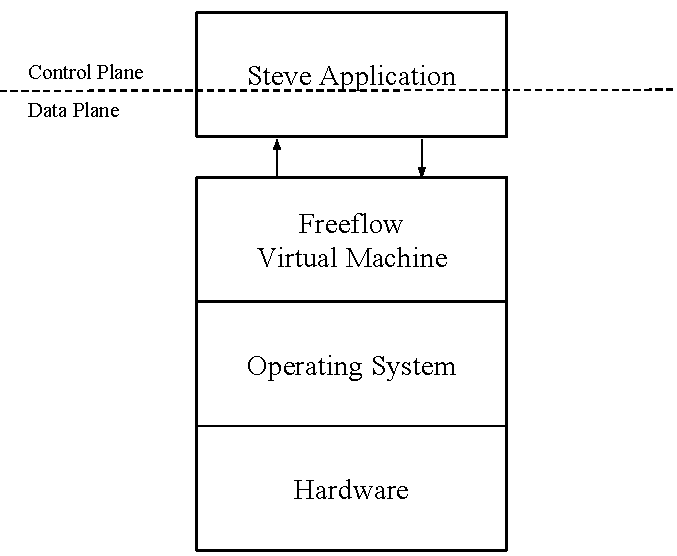
\includegraphics[scale=0.5]{ff_arch}
\caption{The Freeflow System Architecture.}
\label{ff_arch}
\end{figure}

\section{Control Plane}
\label{ff:cp}
The control plane acts as the brain in a network switch, and is responsible for
the hosting of applications as well as the management of the underlying data
plane. In the control plane, the system configuration establishes the resources
that must be provided to support application execution. During execution, events
raised from the data plane are caught and processed by application defined event
handlers.

\section{Data Plane}
\label{ff:dp}
A data plane executes the forwarding behavior for traffic flows using a variety
of hardware, and sometimes software, constructs available in a given system.

\section{Applications}
\label{ff:app}
Freeflow applications provide the logic for the control and data planes in the
switch. This is a departure from common SDN paradigms, where the two planes are
treated as seperate entities and communicate over a secure channel. The reason
for blurring the line between the two parts is to reduce the overhead penalty
that is incurred in the former model. By allowing the application to straddle
the line between the control and data planes, the logic it provides is able
to be pushed into hardware and executed in a native fashion.

\section{Packet Context}
\label{vm:context}
Lots to talk about here.

\section{Virtual Machine}
\label{vm}
The Freeflow Virtual Machine is composed of modular parts that a programmer can
assemble into a virtual switch.

\begin{figure}[h]
\centering
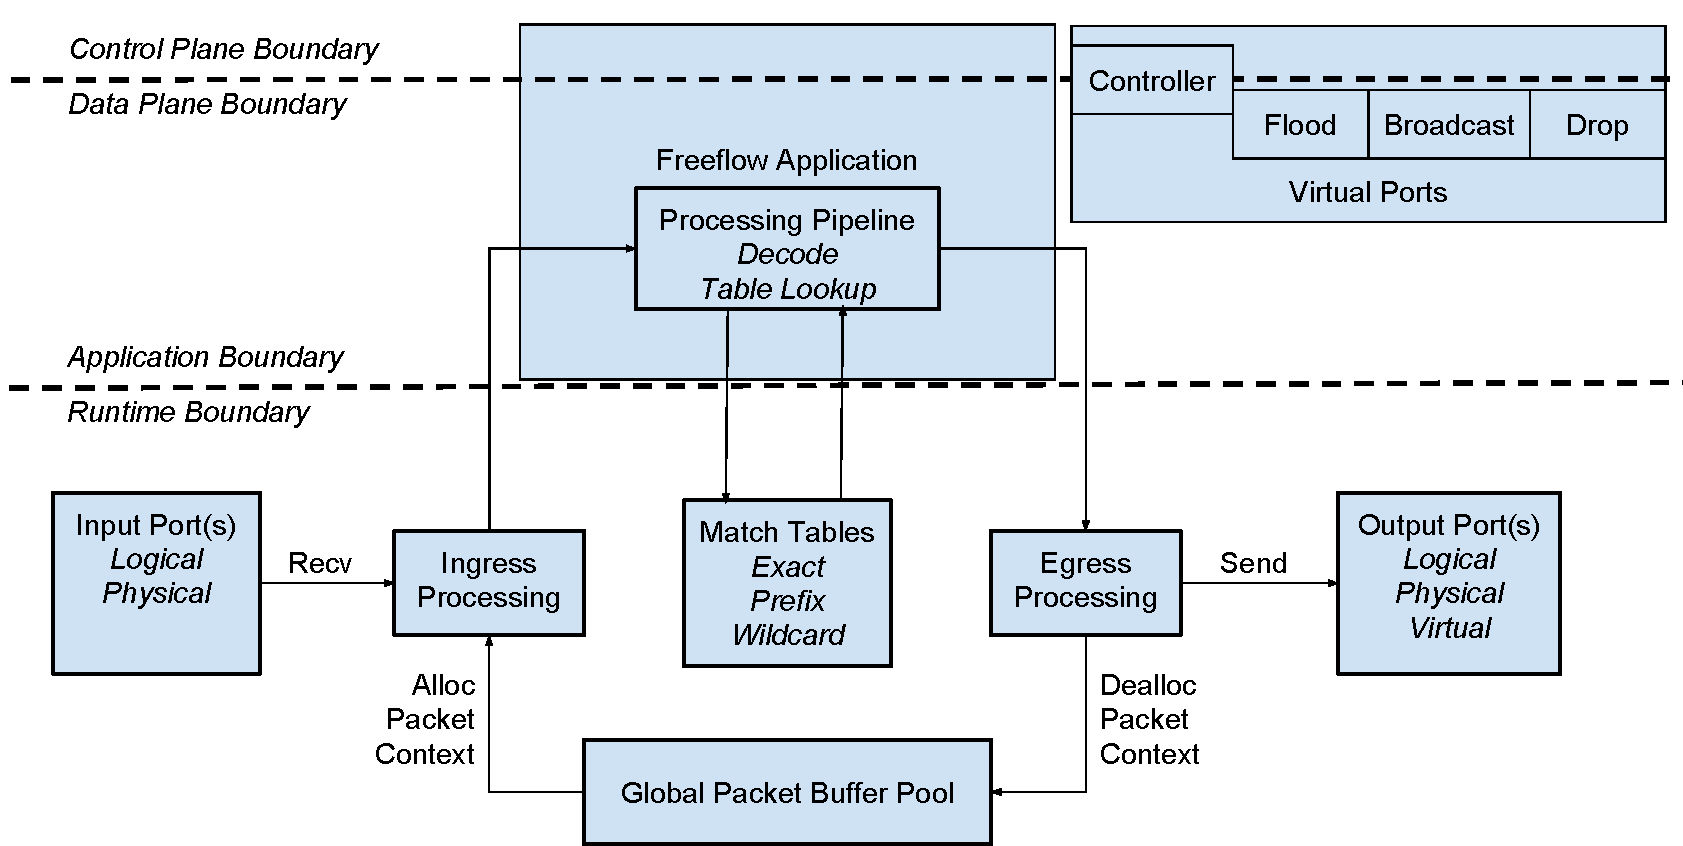
\includegraphics[scale=0.5]{ff_system}
\caption{The Virtual Machine System Architecture}
\label{fig:ff_system}
\end{figure}

\section{Ports}
\label{vm:port}
Ports act as the main source of I/O for network applications. The provide the
means to receive and send packets that are entering and leaving the system. As
an abstract type, the port interface is fairly simple. Any derived port object
needs to implement the following four functions:

\begin{itemize}
\item Send - Transmit packet data.
\item Receive - Retrieve packet data.
\item Up - Puts the port into a usable state, data can be sent and received.
\item Down - Disables port functionality.
\end{itemize}

Port objects can be classified as being either physical, logical, or virtual. A
physical port represents a hardware networking interface, e.g. ethernet cards.
Logical ports represent software networking constructs that utilize file
descriptors to act as a endpoint for communication. An illustration of the port
object UML can be found in figure \ref{port_uml}. Virtual ports are derived
from logical ports, and provide specialized functionality for the system. To
further classify the port type, they can be either seen as an \emph{input} port,
where data from an external source can be injected into the system, or an
\emph{output} port, which sends data to other external or internal devices.

\begin{figure}[h]
\centering
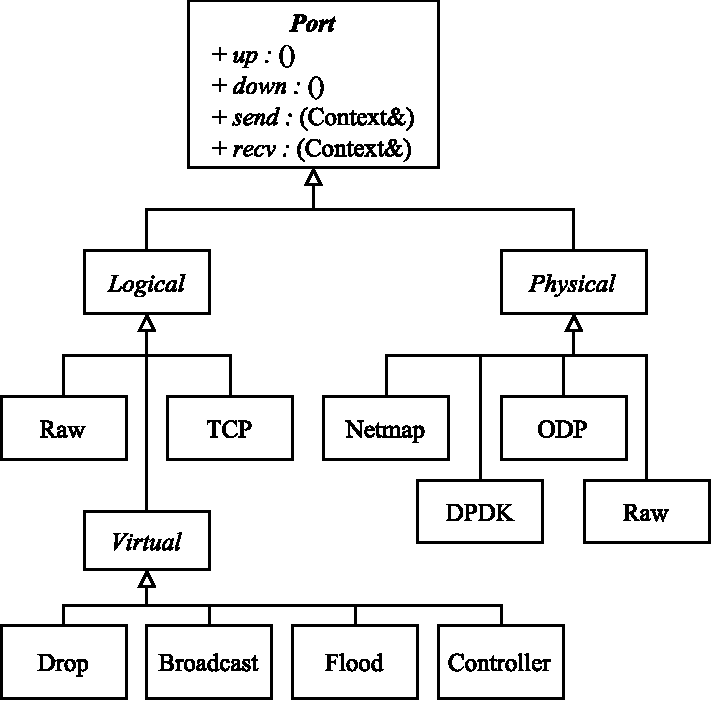
\includegraphics[scale=0.5]{ff_port_uml}
\caption{Freeflow port uml diagaram.}
\label{port_uml}
\end{figure}

\section{Tables}
\label{vm:tables}
In network switches, tables are used to match properties from network flows with
user-defined forwarding behaviors. They can be defined using a variety of
data structures and algorithms to implement them, but generally are categorized
as \emph{exact}, \emph{prefix}, or \emph{wildcard}. Each entry in a flow table
contains a \emph{key}, that is compared to a certain field within packet

The semantics for each of
these matching types are as follows:

Entries in a table contain a \emph{key}, which
is used to aggregate traffic containing similar characteristics into flows.


\section{Instructions}
\label{vm:insn}
Native insn execution. Offloading, optimizations.

\section{Memory}
\label{vm:memory}
Memory model.

\section{Threading}
\label{vm:threading}
Threading models.
